
\begin{figure*}[t]
    \centering
    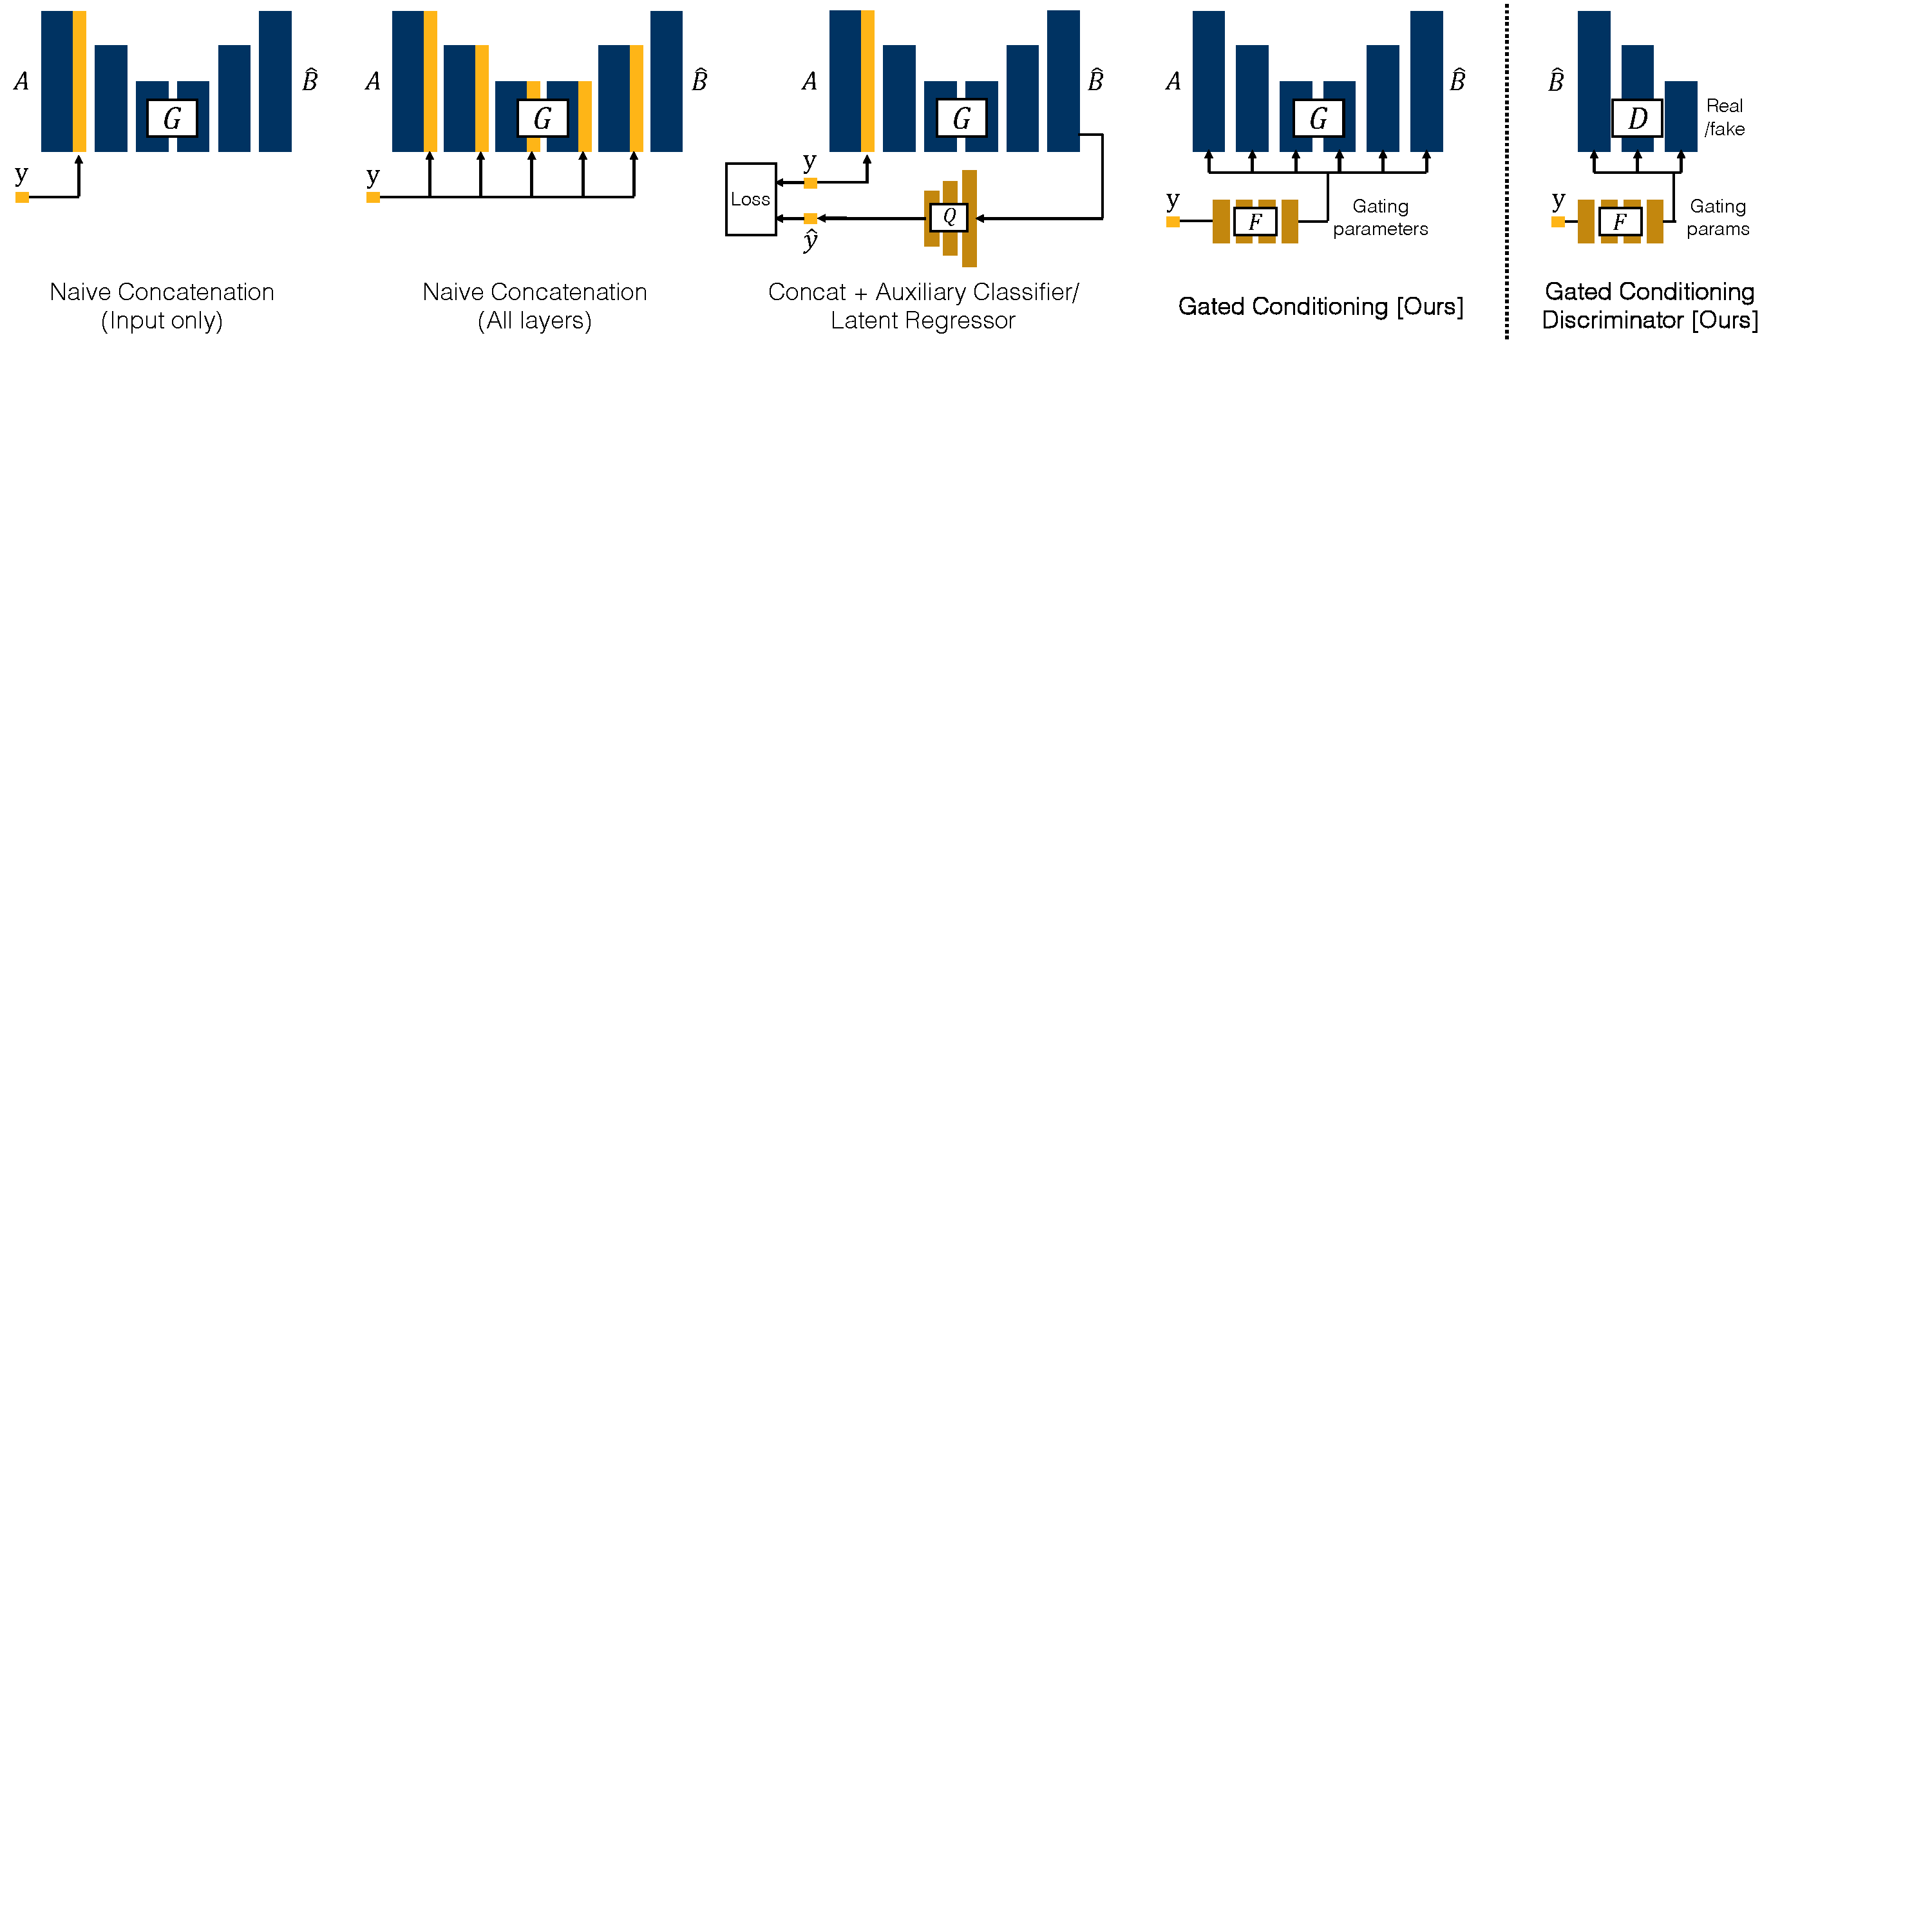
\includegraphics[width=\linewidth]{paper_images/arch_inject.pdf}
    \caption{{\bf Conditioning injection variants.}
    Conditioning information can be incorporated naively in a generator architecture through simple concatenation in {\bf (left)} the input layer only or {\bf (mid-left)} in all layers. {\bf (middle)} The network can be further encouraged to use the conditioning through a learned network, either a classification objective for categorical conditioning~\cite{odena2016conditional,chen2016infogan} or a regression objective for continuous conditioning. {\bf (Mid-right)} We investigate training a network on the conditioning signal, which predicts parameters which are used to guide softly-gated units in the main network. {\bf (Right)} These conditioning options -- concatenation, auxiliary classifier/latent regressor, and our gated conditioning -- can be correspondingly applied to a discriminator.\label{fig:arch-inj} }
    % \vspace{-4mm}
\end{figure*}

\section{Introduction}
Generative methods have made huge strides in the last few years driven by the success of Variational Autoencoders (VAEs)~\cite{kingma2013auto} and Generative Adversarial Networks (GANs)~\cite{goodfellow2014generative}. 
These methods can generate impressive results but one major challenge is that quality degrades quickly when the diversity of training data (e.g., number of object/scene classes) increases. 
It is a common practice in the domain of image conditional generations to train different models for different datasets \cite{goodfellow2014generative,isola2016image2image,karras2017progressive,zhu2017toward,zhu2017unpaired,wang2018video} meaning the number of parameters scales linearly with the number of classes. 
% A study performed in \cite{ghosh2017multi,metz2017unrolledGAN} demonstrated that even in a simple 1D \& 2D Mixture of Gaussians settings, state-of-the-art GAN techniques were not able to generate samples from all the components of the mixture. 
%However their proposed method still involved training multiple generators.
An ideal scenario in such settings would involve a single network which could share parts responsible for similar operations across classes while unsharing the discrete parts of the network which are responsible for class specific operations.

Such a scenario was analyzed in the realm of image classification by Veit et al.~\cite{veit2016residual} where they performed incision experiments on a pretrained ResNet architecture \cite{he2016deep}, demonstrating that certain paths in the network played a more important role for certain classes.
%inferring that ResNets behave like an ensemble of several partially disjoint networks for image classification. 
In this paper we analyze implications of this observation in a generative modeling scenario. 
We analyze GANs on a 1D Mixture of Gaussians dataset as used in \cite{ghosh2017multi}, and discover that the removal of certain blocks of the generator correspond to the disappearance of certain modes in the generated distribution.

Motivated by this, we introduce a simple {\em soft gating} mechanism where based on the conditioning input a hypernetwork predicts which parts of ResNet to use for that particular conditioning.
We explore and analyze different types of gating, including a {\em blockwise} and {\em channelwise} gating, each with multiplicative and affine forms of soft weighting, as well as other related methods like AdaIn~\cite{huang2017arbitrary,huang2018multimodal}, and InfoGAN~\cite{chen2016infogan}. We show that a channelwise multiplicative gating performs best for our task, and better results can be obtained by applying gating not only to the generator but also to the discriminator.


To evaluate our approach, we introduce a new task of generating multi-class images from rough outline scribbles where gating is particularly useful due to class ambiguities in the mapping. Fig.~\ref{fig:teaser} (top left) shows one such example where the same simple scribble yields different outputs of a generator conditioned on ten different classes.
In the unsupervised InfoGAN~\cite{chen2016infogan} setting where classes are not known apriori, conditioning is in the form of a random vector. 
While this scenario was previously shown to produce limited texture variation~\cite{ghosh2017multi} for challenging datasets using naive concatenation-based conditioning, our gating based method is able to produce diverse generations, as shown in Fig.~\ref{fig:teaser} (top right).
In addition, we also evaluate our approach on {\em multi-task image-to-image translation}. 
In its original setting \cite{isola2016image2image}, different trained models were used for each translation tasks. 
Our gating mechanism enables good performance of a single network on multiple tasks by activating appropriate task-specific blocks and channels (Fig.~\ref{fig:teaser} bottom).

%whereby the rough scribbles divulge almost no information about the class.



%%The technique presented a scenario in which we could generate multiple modes for a single dataset but it could further be used for generating multiple modes from a dataset consisting of multiple classes and the hypernetwork could choose the blocks needed for a particular class. 




%%Furthermore we perform a systematic analysis of all meaningful gating mechanisms and other forms of conditioning in the setting of a image conditioned generative model. This paper also finds that gating also enables the discriminator to provide better class conditioned gradients back to the generator for high quality generations.


% Generative methods have made huge strides in the last few years driven by the success of Variational Autoencoders (VAEs)~\cite{kingma2013auto} and Generative Adversarial Networks (GANs)~\cite{goodfellow2014generative}. 
% While these methods can generate impressive results, one major challenge is that quality degrades quickly when the diversity of training data (e.g., number of object/scene classes) increases, especially when the manifold of the multi-class distribution of images drawn from the ground truth distribution is not continuous. \ow{um... I don't really get this previous sentence}

% We propose a solution to generate multi-class images using a form of class conditioning that outperforms prior class conditioned GANs while requiring significantly fewer parameters than using a single GAN per-class. 
% To do this, we take advantage of the fact that different classes will share similar visual features, and propose an architecture wherein a fully-residual GAN generator and discriminator, is combined with a second ``gating'' network, which determines how the network is conditioned on the input class.

% We compare various forms of gating, such as concatenating one-hot class information, auxillary classification, \todo{...}.

% We evaluate our gating approach on a number of applications \todo{...}
% \ow{discuss evaluation and findings}
%



In summary, our contributions are:
\setlength\itemsep{0px}
\begin{itemize}
\itemsep0em 
\item An in-depth analysis of the role of gating networks in generative modeling.
\item A novel architecture using a gating hypernetwork that can generate diverse multi-class results both when classes are known a-priori, or are derived from the data in an unsupervised fashion (similar to InfoGAN~\cite{chen2016infogan}).
%\item Incision experiments on a trained Residual Generator based GAN on the 1D Mixture of Gaussians to show certain blocks correspond to certain modes in the generated distribution.
%\item Introduction of the Gated Residual Blocks and the Hypernetwork to predict the corresponding alphas on the Generator and Discriminator.
\item Introduction of a new image-to-image translation task of generating realistic images from very rough outline scribbles.
\end{itemize}